\documentclass{article}
\usepackage{iclr2027_conference,times}
\usepackage[T1]{fontenc}
\usepackage{lmodern}
\usepackage{hyperref}
\usepackage{url}
\usepackage{booktabs}
\usepackage{array}
\usepackage{float}
\usepackage{microtype}
\usepackage{amsmath,amssymb,amsthm,mathtools}
\usepackage{xcolor}
\usepackage{enumitem}
\usepackage{graphicx}
\usepackage{tikz}
\usetikzlibrary{arrows.meta,positioning}

\newtheorem{theorem}{Theorem}
\newtheorem{proposition}[theorem]{Proposition}
\newtheorem{corollary}[theorem]{Corollary}
\newtheorem{lemma}[theorem]{Lemma}
\newtheorem{definition}[theorem]{Definition}
\newcommand{\R}{\mathbb R}
\newcommand{\N}{\mathbb N}
\newcommand{\E}{\mathbb E}
\newcommand{\cH}{\mathcal H_k}
\newcommand{\cS}{\mathcal S}
\newcommand{\cA}{\mathcal A}
\newcommand{\cZ}{\mathcal Z}
\newcommand{\Bpos}{\mathfrak B_{+}}
\newcommand{\Bsgn}{\mathfrak B_{\pm}}
\newcommand{\Vrkhs}{\mathfrak V}
\newcommand{\Crkhs}{\mathfrak C}
\DeclareMathOperator{\supp}{supp}

\title{Cloned States, Linear Regret:\\A Representation-Invariant Theory of Kernel MDPs}
\author{\textbf{Pahan Dewasurendra} \\ Johns Hopkins University}

\hypersetup{pdftitle={Cloned States, Linear Regret: A Representation-Invariant Theory of Kernel MDPs},pdfauthor={Pahan Dewasurendra},pdfkeywords={kernel reinforcement learning, Markov decision processes, information gain, regret lower bounds, RKHS, representation invariance},pdfsubject={preprint}}
\begin{document}
\maketitle

\begin{abstract}
A common kernel-MDP assumption requires every scalar transition slice
$z\mapsto P_h(s'\mid z)$ to have bounded norm in a state-action RKHS. We show
that this condition measures the names assigned to next states, not the decision
problem. Replacing a state by $m$ behaviorally identical clones divides every
associated slice norm by $m$, while preserving all policy values, every learning
algorithm's attainable observation laws, minimax regret, and the kernel's maximum
information gain. More strongly, we construct a fixed two-step MDP domain and a
fixed Mat\'ern kernel with sublinear information gain for which the coordinatewise
condition, with any prescribed constant, permits linear minimax regret. This gives
a negative answer to the COLT 2024 no-regret open problem under its stated
assumption. We then introduce the \emph{Bellman radius}, the operator norm of the
transition kernel from bounded values to the state-action RKHS. It is invariant to
state cloning, is the exact constant needed for Bellman closure, and is equivalent
up to a factor two to the semivariation of an RKHS-valued transition measure.
An integrable RKHS norm of a transition density is a verifiable stronger condition.
It exposes the missing state-volume factor in the frequently cited coordinatewise
argument. These results separate valid Bellman-closure and conditional-embedding
theorems from representation-dependent sufficient conditions, and give a drop-in
premise for future kernel RL guarantees.
\end{abstract}

\section{Introduction}

Kernel methods offer a natural route from linear reinforcement learning to nonlinear
function approximation. A widely used model assumes that for every next state $s'$,
the scalar function $z\mapsto P_h(s'\mid z)$ belongs to the unit ball of a known
reproducing kernel Hilbert space (RKHS) on state-action pairs
\citep{yang2020kernel,yeh2023sample,vakili2023kernel,
vakili2024rewardfree,vakili2024average,kayal2025rewardfree}.
The intended consequence is that every Bellman image
\begin{equation}
  [P_hV](z)=\int_{\cS}V(s')P_h(ds'\mid z)
  \label{eq:bellman-image}
\end{equation}
also has controlled RKHS norm. Kernel ridge confidence sets can then be applied to
the moving value targets produced by value iteration.

There is a basic obstruction. Split one next-state label into $m$ labels with the
same reward and future dynamics, and allocate one $m$th of its probability to each.
The agent has not received a new control problem. It only observes an independent
uniform label after the transition. Yet all $m$ scalar probability functions now
have one $m$th of the original norm. This operation can make the coordinate bound
arbitrarily small without making learning easier.

The issue is not merely aesthetic. We use state cloning to encode an unrestricted
smooth continuum-armed bandit inside transition probabilities whose individual
RKHS norms are arbitrarily small. The construction uses one fixed countable state
space and one fixed Mat\'ern kernel. Its maximum information gain is sublinear, but
its minimax regret is linear. Thus the coordinatewise premise in the kernel-RL open
problem of \citet{vakili2024open} cannot by itself support no-regret learning.

The right object is already implicit in Bellman's equation. We define
\begin{equation}
 \Bpos(P;\cH)=
 \sup_{V:\,0\leq V\leq1}\|PV\|_{\cH}.
 \label{eq:bellman-radius-intro}
\end{equation}
This \emph{Bellman radius} is unchanged by cloning and is exactly the smallest
constant controlling every bounded nonnegative value image. For discrete states,
its signed counterpart is the semivariation of the RKHS-valued measure
$A\mapsto P(A\mid\cdot)$. For transition densities $p(s'\mid\cdot)$ relative to a
reference measure $\mu$, the stronger quantity
$\int\|p(s'\mid\cdot)\|_{\cH}\,d\mu(s')$ controls the radius. Unlike a pointwise
density bound, this integral retains the state-volume factor and is invariant to a
change of density convention.

\paragraph{Contributions.}
\begin{itemize}[leftmargin=*,itemsep=2pt,topsep=2pt]
  \item We prove an exact state-refinement theorem. State cloning preserves the
  entire projected learning experiment, minimax regret, and maximum information
  gain, while coordinate transition norms decrease by arbitrary factors.
  \item We prove a linear minimax-regret lower bound under the stated assumption of
  \citet{vakili2024open}. The state space, reward, and Mat\'ern kernel are fixed,
  and the kernel has $o(T)$ information gain.
  \item We characterize a representation-invariant replacement through the Bellman
  radius, semivariation, and transition-density variation. The hierarchy gives exact
  Bellman closure and clarifies when coordinate assumptions can be repaired.
  \item We audit the proof-level consequence across kernel-RL results from 2020 to
  2026. Direct Bellman-closure, smooth-Bellman, and bounded conditional-embedding
  results remain intact. Claims that derive closure from coordinate slices require a
  cardinality, volume, or operator-radius term.
\end{itemize}

\begin{figure}[t]
\centering
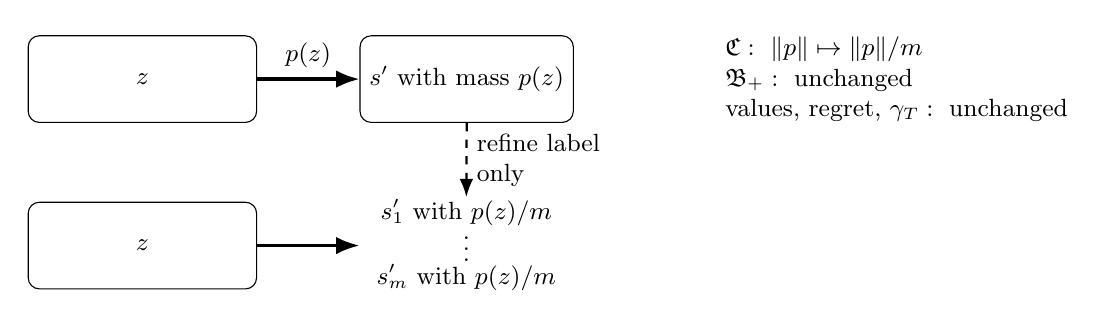
\begin{tikzpicture}[font=\small,>=Latex,node distance=7mm and 13mm]
 \node[draw,rounded corners,minimum width=29mm,minimum height=11mm] (x)
 {$z$};
 \node[draw,rounded corners,right=of x,minimum width=27mm,minimum height=11mm] (y)
 {$s'$ with mass $p(z)$};
 \draw[->,very thick] (x) -- node[above] {$p(z)$} (y);
 \node[below=10mm of x,draw,rounded corners,minimum width=29mm,minimum height=11mm] (xc)
 {$z$};
 \node[right=of xc,inner sep=0] (clones) {\begin{tabular}{c}
 $s'_1$ with $p(z)/m$\\[-1mm] $\vdots$\\[-1mm] $s'_m$ with $p(z)/m$
 \end{tabular}};
 \draw[->,very thick] (xc) -- (clones);
 \draw[->,dashed,thick] (y.south) -- node[right,align=left] {refine label\\only} (clones.north);
 \node[right=18mm of y,align=left] (facts) {
 $\Crkhs:\ \|p\|\mapsto\|p\|/m$\\
 $\Bpos:\ \text{unchanged}$\\
 values, regret, $\gamma_T:\ \text{unchanged}$};
\end{tikzpicture}
\caption{State cloning changes a coordinatewise RKHS parameter without changing
the learning problem. Clone indices are independent random labels.}
\label{fig:cloning}
\end{figure}

\section{Coordinate norms are not properties of an MDP}
\label{sec:cloning}

Let $P$ be a Markov kernel from a current state-action domain $\cZ$ to a finite or
countable next-state space $\cS$. Let $k$ be a kernel on $\cZ$ with RKHS $\cH$.
Write $p_y=P(\{y\}\mid\cdot)$ and define the coordinate radius
\begin{equation}
 \Crkhs(P;\cH)=\sup_{y\in\cS}\|p_y\|_{\cH}.
 \label{eq:coordinate-radius}
\end{equation}
This is the premise in \citet{vakili2024open}, up to a constant $u$.

Choose integers $m_y\geq1$. The refined state space is
$\widetilde\cS=\{(y,i):y\in\cS,\ i\in[m_y]\}$ and the refined transition is
\begin{equation}
 \widetilde P((y,i)\mid z)=\frac{P(y\mid z)}{m_y}.
 \label{eq:clone-transition}
\end{equation}
For a full MDP, rewards and future transitions are constant within each fiber.
If current states are also refined, use the pulled-back kernel
$\widetilde k((s,i,a),(s',j,a'))=k((s,a),(s',a'))$.

\begin{theorem}[Exact state refinement]
\label{thm:refinement}
For any episodic MDP and any finite clone counts, the refined MDP has the following
properties. The regret statement applies to any model family and its paired family
of refinements.
\begin{enumerate}[leftmargin=*,itemsep=2pt,topsep=2pt]
 \item Projection of a refined trajectory onto original state labels has the
 original trajectory law. Conversely, every policy using clone labels can be
 simulated in the original MDP using private randomization. Hence paired policies
 have identical value and regret laws, and paired model families have the same
 minimax regret for every number of episodes.
 \item The pulled-back RKHS is isometric to the original RKHS and
 \begin{equation}
   \Crkhs(\widetilde P;\widetilde\cH)
   =\sup_{y\in\cS}\frac{\|p_y\|_{\cH}}{m_y}.
   \label{eq:coordinate-shrink}
 \end{equation}
 \item For every regularization $\lambda>0$ and budget $T$, the maximum information
 gain satisfies $\gamma_T(\widetilde k;\lambda)=\gamma_T(k;\lambda)$.
\end{enumerate}
\end{theorem}

The proof couples clone indices as independent uniforms and observes that every
refined Gram matrix equals the Gram matrix of its projection. Full details, including
history-dependent randomized policies, are in Appendix~\ref{app:refinement}.
The result is an exact bisimulation-style refinement
\citep{givan2003equivalence}, strengthened here to equality of the sequential
learning experiments and kernel complexity.

\begin{corollary}[Vacuity under finite refinement]
\label{cor:vacuity}
Let a finite MDP have a finite state-action domain and let $k$ be strictly positive
definite on that domain. For every $\epsilon>0$, there is a behaviorally equivalent
refinement with a pulled-back kernel satisfying
$\Crkhs(\widetilde P_h;\widetilde\cH)\leq\epsilon$ for every stage $h$. Rewards keep
their RKHS norms and every $\gamma_T$ is unchanged.
\end{corollary}

Every function on a finite domain belongs to the RKHS of a strictly positive
definite Gram matrix. Choosing $m_y$ large enough proves the corollary. Therefore a
uniform coordinate bound can certify every finite decision problem after harmless
state refinement. The next result rules out the objection that the pulled-back
kernel is responsible.

\section{A fixed Mat\'ern kernel still permits linear regret}
\label{sec:lower}

We consider the online episodic setting of \citet{vakili2024open}. Rewards are
deterministic and known, transitions are unknown, and regret after $T$ episodes is
$R_T=\sum_{t=1}^T(V_1^*-V_1^{\pi_t})$. The assumption is that a known kernel $k$
satisfies $\|P_h(s'\mid\cdot)\|_{\cH}\leq u$ for every $h$ and $s'$, where $u>0$
is fixed.

\begin{theorem}[No uniform no-regret under coordinate smoothness]
\label{thm:linear}
Fix any $u>0$ and any Mat\'ern smoothness $\nu>1/2$. There exist a fixed compact
state-action domain $\cZ$, a fixed countable state space, a fixed known reward, and
the restriction to $\cZ$ of a unit-variance Mat\'ern kernel on $[0,1]^2$ such that
\begin{equation}
 \inf_{\mathsf A}\ \sup_{M:\,\Crkhs(P_h;\cH)\leq u}
 \E_M[R_T(\mathsf A)]\ \geq c_\nu T
 \qquad\text{for every }T\geq2,
 \label{eq:linear-regret}
\end{equation}
where $c_\nu>0$ does not depend on $T$. At the same time,
$\gamma_T(k;1)=\widetilde O(T^{2/(2\nu+2)})=o(T)$.
The claim already holds for horizon two.
\end{theorem}

\paragraph{Construction and proof idea.}
At the first stage there is one state and the action is $x\in[0,1]$. Terminal
states are fixed labels $\{g_n,b_n:n\in\N\}$, with known rewards $\alpha$ and zero.
For $M=2T$, place smooth unit-height bumps $\psi_1,\ldots,\psi_M$ on disjoint
intervals. Instance $j$ has total probability
\begin{equation}
 f_j(x)=\tfrac12+\Delta\psi_j(x)
 \label{eq:bump-mean}
\end{equation}
of reaching a good state. Spread this mass uniformly across $N_T$ good labels and
the complementary mass across $N_T$ bad labels. Each scalar transition function is
therefore $f_j/N_T$ or $(1-f_j)/N_T$. Smooth compactly supported functions belong
to every finite-smoothness Mat\'ern RKHS on a compact domain
\citep{wendland2005scattered,kanagawa2018review}. A finite $N_T$ can consequently
make every slice norm at most $u$, even though the Bellman image remains
$\alpha f_j$.

Under the flat instance $f_0=1/2$, a length-$T$ action sequence can enter at most
$T$ of the $2T$ disjoint supports. A uniformly random support is never entered with
probability at least $1/2$. Until entry, the complete labeled observation history
has the same distribution under $f_j$ and $f_0$. Hence some $j$ is never entered
with probability at least $1/2$ under its own instance. On that event all $T$
actions have gap $\alpha\Delta$, proving
$\E R_T\geq\alpha\Delta T/2$. Appendix~\ref{app:lower} gives the formal coupling,
one common Mat\'ern-domain embedding for all stages, and the randomized-algorithm
argument. The standard Mat\'ern information-gain bound gives the final claim
\citep{vakili2021information,janz2020matern}.

The hard MDP may depend on $T$, as is standard in minimax regret. The state space,
kernel, reward, horizon, and coordinate constant do not. The number of labels with
positive transition mass grows with $T$. This is precisely the degree of freedom
left uncontrolled by the coordinate assumption. Theorem~\ref{thm:linear} gives a
negative answer to the no-regret part of the COLT 2024 open problem \emph{under its
stated Assumption 1}. It does not rule out no-regret guarantees under direct Bellman
closure, a fixed finite cardinality, or smooth transition densities with controlled
integrated norm.

\section{The representation-invariant quantity}
\label{sec:radius}

For a transition kernel $P$ whose relevant Bellman images belong to $\cH$, define
the positive and signed Bellman radii
\begin{equation}
 \Bpos(P;\cH)=\sup_{0\leq V\leq1}\|PV\|_{\cH},
 \qquad
 \Bsgn(P;\cH)=\sup_{\|V\|_\infty\leq1}\|PV\|_{\cH}.
 \label{eq:radii}
\end{equation}
For countable states, also define the RKHS slice variation
\begin{equation}
 \Vrkhs(P;\cH)=\sum_{y\in\cS}\|p_y\|_{\cH}.
 \label{eq:variation}
\end{equation}

\begin{theorem}[Radius hierarchy and invariance]
\label{thm:radius}
Whenever the quantities are finite,
\begin{equation}
 \Crkhs(P;\cH)\leq\Bpos(P;\cH)
 \leq\Bsgn(P;\cH)\leq2\Bpos(P;\cH)
 \leq2\Vrkhs(P;\cH).
 \label{eq:hierarchy}
\end{equation}
Both Bellman radii and the slice variation are exactly invariant under arbitrary
state-dependent cloning. The positive radius is the smallest $B$ such that
$\|PV\|_{\cH}\leq B\|V\|_\infty$ for every nonnegative bounded $V$. The signed
radius is the semivariation of the $\cH$-valued transition measure
$A\mapsto P(A\mid\cdot)$ whenever this set function is countably additive in
$\cH$ \citep{diestel1977vector}.
No reverse inequality in equation~\eqref{eq:hierarchy} is dimension free.
\end{theorem}

The invariance proof is exact. For a function $\widetilde V$ on clones, let
$\bar V(y)=m_y^{-1}\sum_i\widetilde V(y,i)$. Then
$\widetilde P\widetilde V=P\bar V$, and every $V$ has a constant-on-fibers lift.
The variation identity follows by summing $m_y$ copies of
$\|p_y/m_y\|_{\cH}$. The factor-two equivalence uses
$V=V_+-V_-$ for signed $V$. Examples in Appendix~\ref{app:radius} show strict
separations of order $n$ and $\sqrt n$ between the three quantities.

The hierarchy also clarifies transition densities. Suppose
$P(ds'\mid z)=p(s'\mid z)\mu(ds')$ and
$s'\mapsto p(s'\mid\cdot)$ is Bochner integrable in $\cH$.

\begin{proposition}[Density variation]
\label{prop:density}
Define
\begin{equation}
 \Vrkhs_\mu(P;\cH)=
 \int_{\cS}\|p(s'\mid\cdot)\|_{\cH}\,d\mu(s').
 \label{eq:density-variation}
\end{equation}
Then $\Bpos(P;\cH)\leq\Vrkhs_\mu(P;\cH)$. If
$\|p(s'\mid\cdot)\|_{\cH}\leq u$ pointwise, the valid conclusion is
$\Bpos(P;\cH)\leq u\mu(\cS)$. The quantity in
equation~\eqref{eq:density-variation} is unchanged under equivalent changes of
reference measure and measurable relabelings.
\end{proposition}

The proof is the Bochner triangle inequality. Under $d\mu'=w,d\mu$, the new
density is $p'=p/w$, so the integrated norm is unchanged. A pointwise density
constant alone is therefore incomplete without the reference-measure mass. This
matches the general $L^\infty\!\to\cH$ conditional-expectation criterion noted by
\citet{hertel2026regularity}. Their broader operator theory treats $L^p$ domains,
density regularity, and conditional mean embeddings. Our Bellman radius is the
exact intrinsic norm for bounded RL value functions.

\begin{corollary}[Exact Bellman closure]
\label{cor:closure}
If $\|r_h\|_{\cH}\leq B_r$ and
$\Bpos(P_h;\cH)\leq B_P$, then for every $V:\cS\to[0,H-h]$,
\begin{equation}
 \|r_h+P_hV\|_{\cH}\leq B_r+(H-h)B_P.
 \label{eq:closure}
\end{equation}
Conversely, with $r_h=0$, the smallest uniform constant in
equation~\eqref{eq:closure} is $(H-h)\Bpos(P_h;\cH)$.
\end{corollary}

This is the nonlinear analogue of the integrated vector-measure bound imposed in
linear MDPs \citep{jin2020linear}. It is also the premise actually needed when a
kernel ridge confidence theorem is applied to Bellman targets. Any proof using
coordinate smoothness only through this target-norm step can replace it by
Corollary~\ref{cor:closure}, with the confidence radius scaled by
$B_r+HB_P$.

\section{What changes in existing kernel RL theory}
\label{sec:audit}

Table~\ref{tab:audit} separates three assumptions that are often described with
similar language. They are not equivalent.

\begin{table}[H]
\centering
\small
\setlength{\tabcolsep}{4pt}
\begin{tabular}{>{\raggedright\arraybackslash}p{0.22\linewidth}
                >{\raggedright\arraybackslash}p{0.31\linewidth}
                >{\raggedright\arraybackslash}p{0.39\linewidth}}
\toprule
Work & Formal premise or proof step & Consequence of our results \\
\midrule
\citet{yang2020kernel}
& Main theorem assumes bounded Bellman images directly. A separate paragraph says coordinate slices suffice.
& The theorem under direct closure is unchanged. The stated sufficient condition needs slice variation or a finite volume factor. \\
\citet{yeh2023sample}
& Coordinate density norm at most one. Lemma 3 proves $\|PV\|\leq c\|V\|_\infty$, where $c=\int_{\cS}ds'$.
& The proof correctly retains state volume $c$. Omitting $c$ in later uses is not representation invariant. \\
\citet{vakili2024rewardfree}
& Lemma 2.3 invokes the same calculation for values on the Lebesgue unit cube.
& This normalized specialization is valid because the reference volume is one. \\
\citet{vakili2023kernel,vakili2024average,vakili2024open}
& Coordinate masses or densities are bounded, followed by a dimension-free Bellman-target claim.
& That implication fails on general state spaces. Theorem~\ref{thm:linear} rules out uniform no-regret under the open problem's stated premise. \\
\citet{kayal2025rewardfree,cioba2026invariances,pavlovic2026preferences}
& Recent uses cite the same coordinate-to-Bellman implication with an $O(H)$ radius.
& The hidden constant must include volume, variation, or $\Bpos$. Other parts of the analyses may remain applicable after this replacement. \\
\citet{maran2024local,maran2024smooth}
& Smoothness or local linearity is imposed on Bellman images. Appendix F of the latter identifies a separate localization issue in \citet{vakili2023kernel}.
& These structural premises are clone invariant and are not targeted by our lower bound. \\
\citet{chowdhury2023cme,kumar2025closure}
& A bounded conditional mean embedding operator is assumed. The latter work enforces a state-RKHS ball by projection.
& These are operator-level, representation-invariant alternatives, though they control a specified state-function RKHS rather than all bounded values. \\
\bottomrule
\end{tabular}
\caption{Proof-level audit. ``Unchanged'' refers only to the issue studied here.
All original auxiliary conditions are still required.}
\label{tab:audit}
\end{table}

The most precise source for the frequently cited calculation is
\citet[Lemma 3]{yeh2023sample}. Its proof integrates the pointwise RKHS norm and
obtains $c=\int_{\cS}ds'$, exactly as Proposition~\ref{prop:density} predicts.
For a counting measure, $c=|\cS|$. Under $m$-fold cloning the pointwise coordinate
norm falls by $m$ and $c$ grows by $m$, leaving the product unchanged. Treating $c$
as a universal constant removes the compensating term.

There are two clean routes forward. One can assume the Bellman radius directly,
which is minimal for bounded value iteration. Alternatively, one can verify a
stronger integrated density or conditional-operator condition. Recent work on
conditional expectations provides analytic density criteria
\citep{park2020measure,hertel2026regularity}, while CME-based RL uses a bounded
operator between chosen RKHSs \citep{chowdhury2023cme,kumar2025closure}. The recent
projection approach enforces membership in its chosen state-RKHS ball. It does not
analyze coordinate slices or all bounded value functions. Smooth-MDP analyses impose
regularity on the Bellman operator itself \citep{maran2024local,maran2024smooth}.
Kernel smoothing of a transition distribution is another distinct model and does
not rely on coordinate masses \citep{domingues2021kernel}.

\section{Discussion and limitations}

State representations are rarely canonical. Equivalent states can arise from
tokenization, redundant simulator variables, duplicated observations, or a refined
discretization. A structural complexity parameter should not improve merely because
such labels are duplicated. Coordinatewise probability masses fail this test.
Pointwise transition \emph{densities} can still be meaningful when a canonical
reference measure and its volume are part of the model. The distinction must be
explicit.

Our lower bound is uniform minimax rather than a single fixed instance with linear
asymptotic regret. It exploits an unbounded number of active clone labels, which is
allowed by the stated premise. Fixed finite state cardinality restores a factor
$|\cS|$ and does not contradict tabular learning. We do not propose a new RL
algorithm, and a small Bellman radius may itself be difficult to verify from data.
The result instead identifies the weakest norm premise needed by a broad family of
kernel value-iteration proofs and supplies verifiable stronger conditions.

The conclusion is narrow but consequential. Sublinear kernel information gain
describes how well fixed RKHS functions can be learned. It cannot guarantee that
the moving Bellman targets have bounded RKHS norm. That second property belongs to
the transition operator, not to its individual coordinates.

\subsection*{Ethics statement}

This theoretical work uses no human-subject data and introduces no direct societal
risk. Its audit of prior claims is phrased at the level of assumptions and proof
steps. We distinguish unaffected theorems from affected sufficient conditions.

\subsection*{Reproducibility statement}

Appendices~\ref{app:refinement}--\ref{app:checks} contain complete proofs and the
fixed-domain lower-bound construction. The supplementary artifact verifies cloning
identities, the radius hierarchy on finite kernels, and the hard-instance coupling
by exact enumeration. It uses only standard Python and NumPy.

\bibliography{references}
\bibliographystyle{iclr2027_conference}

\appendix
\section{Notation and technical preliminaries}
\label{app:prelim}

For an episodic MDP, $h\in[H]$ indexes the stage, $s\in\cS$ the state,
$a\in\cA$ the action, and $z=(s,a)\in\cZ$. Rewards lie in $[0,1]$.
Policies and learning algorithms may be randomized and history dependent. The
kernel $k$ is positive semidefinite and has RKHS $\cH$. Its maximum information
gain at regularization $\lambda>0$ is
\begin{equation}
 \gamma_T(k;\lambda)=
 \sup_{z_1,\ldots,z_T\in\cZ}
 \frac12\log\det(I_T+\lambda^{-1}K_T),
 \qquad [K_T]_{ij}=k(z_i,z_j).
 \label{eq:gamma-app}
\end{equation}
We allow repeated points in the supremum. This convention has no effect on the
arguments.

We use the following elementary pullback fact.

\begin{lemma}[Pullback RKHS]
\label{lem:pullback}
Let $q:\widetilde\cZ\to\cZ$ be surjective and let
$\widetilde k(\tilde z,\tilde z')=k(q(\tilde z),q(\tilde z'))$. Then
\begin{equation}
 \widetilde\cH=\{f\circ q:f\in\cH\},
 \qquad \|f\circ q\|_{\widetilde\cH}=\|f\|_{\cH}.
 \label{eq:pullback-isometry}
\end{equation}
Also $\gamma_T(\widetilde k;\lambda)=\gamma_T(k;\lambda)$.
\end{lemma}

\begin{proof}
If $\phi:\cZ\to\mathcal F$ is a feature map for $k$, then
$\widetilde\phi=\phi\circ q$ is a feature map for $\widetilde k$. Surjectivity
means the closed linear spans of $\phi(\cZ)$ and
$\widetilde\phi(\widetilde\cZ)$ coincide. Their canonical feature-space
representations therefore give equation~\eqref{eq:pullback-isometry}. Every
$T$-point Gram matrix in the refined domain is the Gram matrix of its projected
points. Conversely, every original sequence has a lift because $q$ is surjective.
The two suprema in equation~\eqref{eq:gamma-app} are equal.
\end{proof}

\section{Proofs for exact state refinement}
\label{app:refinement}

We first state the full MDP construction. For clarity, take a layered MDP, so a
state cannot occur at two different stages. This loses no generality because the
stage can be appended to the state. For every $s\in\cS_h$, choose a finite integer
$m_s\geq1$ and let
\begin{equation}
 \widetilde\cS_h=\{(s,i):s\in\cS_h,\ i\in[m_s]\}.
\end{equation}
If the original initial distribution is $\rho$, set
$\widetilde\rho(s,i)=\rho(s)/m_s$. Define
\begin{align}
 \widetilde r_h((s,i),a)&=r_h(s,a),
 \label{eq:refined-reward-app}\\
 \widetilde P_h((s',j)\mid(s,i),a)
 &=\frac{P_h(s'\mid s,a)}{m_{s'}}.
 \label{eq:refined-p-app}
\end{align}
The projection $q(s,i)=s$ is a probabilistic bisimulation map.

\subsection{Equality of decision and learning experiments}

Given an original policy $\pi$, define its lift by ignoring clone indices. Summing
equation~\eqref{eq:refined-p-app} over $j$ proves inductively that the projected
trajectory has the original law. Rewards agree pathwise under projection.

The converse must account for a refined policy that uses clone indices. An agent in
the original MDP can generate them privately. At the initial state $s_1$, draw
$I_1$ uniformly from $[m_{s_1}]$. After observing each subsequent original state
$s_h$, draw $I_h$ independently and uniformly from $[m_{s_h}]$. Feed the synthetic
history $((s_1,I_1),a_1,\ldots,(s_h,I_h))$ to the refined policy. Conditional on
the projected history, equation~\eqref{eq:refined-p-app} makes the actual clone
index in the refined MDP exactly independent and uniform. Induction therefore
couples the full reward and projected-state laws.

The same simulation applies across episodes and to a learning algorithm whose next
policy depends on all earlier observations. One direction projects observations.
The other supplies private clone indices. Thus the sets of attainable reward laws
are identical. Optimal values are identical as a special case. Since regret is a
function of the selected-policy values and optimal values, the minimax regret is
identical for every interaction budget. This proves part 1 of
Theorem~\ref{thm:refinement}.

\subsection{Coordinate norm and information gain}

At a transition into $s'$, each refined coordinate function is
\begin{equation}
 \widetilde p_{s',j}((s,i),a)
 =\frac{1}{m_{s'}}p_{s'}(s,a).
\end{equation}
Lemma~\ref{lem:pullback} and homogeneity of the RKHS norm give
\begin{equation}
 \|\widetilde p_{s',j}\|_{\widetilde\cH}
 =\frac{\|p_{s'}\|_{\cH}}{m_{s'}}.
\end{equation}
Taking the supremum proves equation~\eqref{eq:coordinate-shrink}.
The information-gain claim is Lemma~\ref{lem:pullback}. This completes the proof of
Theorem~\ref{thm:refinement}.

\subsection{Proof of Corollary~\ref{cor:vacuity}}

On a finite domain, strict positive definiteness means the Gram matrix is
invertible. Every scalar function $f$ belongs to the RKHS and has finite norm
$\|f\|_{\cH}^2=f^\top K^{-1}f$. There are finitely many stages and target states.
Choose
\begin{equation}
 m_y\geq\max_h\frac{\|P_h(y\mid\cdot)\|_{\cH}}{\epsilon}
\end{equation}
and round upward. Theorem~\ref{thm:refinement} gives the coordinate bound and all
invariances. A pulled-back reward has the same norm by
Lemma~\ref{lem:pullback}.

\section{Proof of the linear-regret theorem}
\label{app:lower}

This section gives one domain and one kernel shared by every interaction budget.
The additional geometric detail ensures that all transition coordinates, including
their values on state-action pairs that are unreachable at a given stage, are
restrictions of Mat\'ern RKHS functions.

\subsection{A fixed compact state-action domain}

Let
\begin{equation}
 \cS=\{s_0,g_\infty,b_\infty\}
 \cup\{g_n,b_n:n\in\N\},
 \qquad \cA=[0,1].
\end{equation}
Assign state coordinates
\begin{align}
 \eta(s_0)&=0,\\
 \eta(g_\infty)&=\tfrac13,
 &\eta(g_n)&=\tfrac13+\frac{1}{100(n+1)},\\
 \eta(b_\infty)&=\tfrac23,
 &\eta(b_n)&=\tfrac23+\frac{1}{100(n+1)}.
\end{align}
Embed $z=(s,a)$ as $\iota(z)=(a,\eta(s))\in[0,1]^2$. The image $\iota(\cZ)$
is compact because both limit-state lines are included. Let $\kappa_\nu$ be the
unit-variance Mat\'ern kernel of smoothness $\nu>1/2$ on $[0,1]^2$ and define
\begin{equation}
 k(z,z')=\kappa_\nu(\iota(z),\iota(z')).
 \label{eq:matern-pullback}
\end{equation}
The embedding is injective, so this is simply the restriction of a fixed Mat\'ern
kernel to a compact subdomain.

Choose $q\in C^\infty([0,1])$ that equals one on the set of good-state
coordinates and zero on the initial and bad-state coordinates. Such a function
exists because these compact sets are separated. The function
$Q(a,y)=q(y)$ has a smooth compactly supported extension to $\R^2$. Mat\'ern RKHSs
on bounded Lipschitz domains are norm equivalent to Sobolev spaces of finite order
\citep{wendland2005scattered,kanagawa2018review}. Hence the restriction of $Q$ to
$\iota(\cZ)$ has a finite RKHS norm $C_q$. Set
\begin{equation}
 \alpha=\min\{1,C_q^{-1}\}>0,
 \qquad r_1\equiv0,
 \qquad r_2(s,a)=\alpha q(\eta(s)).
 \label{eq:fixed-reward}
\end{equation}
The reward is fixed, known, in $[0,1]$, and has RKHS norm at most one. This reward
smoothness is not needed by the open problem, but shows the lower bound survives
the reward part of the stronger coordinate assumptions used elsewhere.

\subsection{The transition family}

Fix $T\geq2$, set $M=2T$, and choose pairwise disjoint open intervals
$I_1,\ldots,I_M\subset(0,1)$. Let
$\psi_j\in C_c^\infty(I_j)$ satisfy $0\leq\psi_j\leq1$ and
$\max_x\psi_j(x)=1$. Let $\Delta=1/4$.

Choose a smooth cutoff $\chi:[0,1]\to[0,1]$ that equals one at zero and equals
zero on every good and bad state coordinate. For $j\in[M]$, define the smooth
ambient functions
\begin{equation}
 F_{j,+}(a,y)=\frac12+\Delta\chi(y)\psi_j(a),
 \qquad
 F_{j,-}(a,y)=\frac12-\Delta\chi(y)\psi_j(a).
 \label{eq:ambient-functions}
\end{equation}
Their restrictions to $\iota(\cZ)$ have finite $\cH$ norms. Put
\begin{equation}
 A_T=\max\left\{
  \max_{j\in[M],\,\sigma\in\{+,-\}}\|F_{j,\sigma}|_{\iota(\cZ)}\|_{\cH},
  \tfrac12\|1\|_{\cH}
 \right\}<\infty
\end{equation}
and choose the integer
\begin{equation}
 N_T\geq A_T/u.
 \label{eq:clone-number}
\end{equation}
The stage-one transitions of instance $j$ are, for every $z=(s,a)$,
\begin{align}
 P_{1,j}(g_n\mid z)&=\frac{F_{j,+}(a,\eta(s))}{N_T},
 &n&\leq N_T,\label{eq:hard-good}\\
 P_{1,j}(b_n\mid z)&=\frac{F_{j,-}(a,\eta(s))}{N_T},
 &n&\leq N_T.\label{eq:hard-bad}
\end{align}
All remaining target states have probability zero. The two displayed families sum
to one and are nonnegative. At stage two, let the transition be independent of
$z$ and uniform on $\{g_n,b_n:n\leq N_T\}$. These final transitions do not affect
return, but they make the coordinate assumption valid for every $h\in[H]$ under
the convention that $P_H$ is specified.

Equations~\eqref{eq:ambient-functions}--\eqref{eq:clone-number} give
\begin{equation}
 \|P_{h,j}(s'\mid\cdot)\|_{\cH}\leq u
 \qquad\text{for every }h\in\{1,2\},\ s'\in\cS.
 \label{eq:coordinate-verified}
\end{equation}
When starting at $s_0$, the total probability of a good terminal state is
\begin{equation}
 \sum_{n\leq N_T}P_{1,j}(g_n\mid(s_0,a))
 =\frac12+\Delta\psi_j(a).
\end{equation}
The episode's expected return is therefore
$\alpha(1/2+\Delta\psi_j(a))$, whose optimum is
$\alpha(1/2+\Delta)$.

The flat instance $0$ replaces every $\psi_j$ by zero and uses the same $N_T$.
Conditioned on ``good'' or ``bad'', the observed index $n$ is uniform on
$[N_T]$ under every instance. Thus the label contains no information beyond the
Bernoulli outcome.

\subsection{Coupling and regret}

Fix an arbitrary randomized history-dependent algorithm $\mathsf A$. Under the flat
instance, let $A_t$ be its first-stage action in episode $t$. For each $j$, define
\begin{equation}
 \tau_j=\inf\{t\leq T:A_t\in\supp(\psi_j)\},
\end{equation}
with $\inf\varnothing=\infty$. For every realized trajectory of actions,
\begin{equation}
 \sum_{j=1}^{M}\mathbf 1\{\tau_j\leq T\}\leq T
 \label{eq:path-hit-count}
\end{equation}
because the supports are disjoint. Taking expectations under the flat instance
and dividing by $M=2T$ gives
\begin{equation}
 \frac1M\sum_{j=1}^M\Pr_0(\tau_j\leq T)\leq\frac12.
 \label{eq:average-hit}
\end{equation}

For a fixed $j$, couple instance $j$ and the flat instance with the same algorithm
randomness and the same random bits used to draw terminal outcomes. Before an
action enters $\supp(\psi_j)$, the good probability is $1/2$ in both instances,
and the conditional clone label is uniform in both. Their histories and next
actions consequently agree until entry. Entry is determined by the action before
the new outcome is observed. Therefore
\begin{equation}
 \Pr_j(\tau_j\leq T)=\Pr_0(\tau_j\leq T).
 \label{eq:hitting-coupling}
\end{equation}
Equation~\eqref{eq:average-hit} supplies some $j^*$ with
$\Pr_{j^*}(\tau_{j^*}>T)\geq1/2$. On this event every selected action has expected
gap $\alpha\Delta$. The expected realized pseudo-regret equals the standard
value regret by the tower property, so
\begin{equation}
 \E_{j^*}R_T
 =\E_{j^*}\sum_{t=1}^T\alpha\Delta(1-\psi_{j^*}(A_t))
 \geq\frac{\alpha\Delta}{2}T.
 \label{eq:lower-complete}
\end{equation}
The argument already includes the algorithm's private randomness and proves the
minimax claim with $c_\nu=\alpha\Delta/2$.

Finally, every Gram matrix of $k$ is a Gram matrix of the ambient Mat\'ern kernel on
$[0,1]^2$. Hence
\begin{equation}
 \gamma_T(k;1)\leq\gamma_T(\kappa_\nu;1)
 =\widetilde O\!\left(T^{2/(2\nu+2)}\right)=o(T),
\end{equation}
using the standard Mat\'ern information-gain bound
\citep{vakili2021information}. This completes the proof of
Theorem~\ref{thm:linear}.

\section{Proofs and separations for Bellman radii}
\label{app:radius}

\subsection{Proof of Theorem~\ref{thm:radius}}

For any state $y$, take $V=\mathbf1_{\{y\}}$ in
equation~\eqref{eq:radii}. This gives $\Crkhs\leq\Bpos$. The inclusion of the
positive unit cube in the signed unit ball gives $\Bpos\leq\Bsgn$.
For any $V$ with $\|V\|_\infty\leq1$, write $V=V_+-V_-$, where
$0\leq V_+,V_-\leq1$. Then
\begin{equation}
 \|PV\|_{\cH}\leq\|PV_+\|_{\cH}+\|PV_-\|_{\cH}
 \leq2\Bpos(P;\cH).
\end{equation}
For $0\leq V\leq1$ on a countable space, the triangle inequality gives
\begin{equation}
 \|PV\|_{\cH}
 =\left\|\sum_yV(y)p_y\right\|_{\cH}
 \leq\sum_yV(y)\|p_y\|_{\cH}
 \leq\Vrkhs(P;\cH).
\end{equation}
Taking suprema proves equation~\eqref{eq:hierarchy}.

For cloning, let
$\bar V(y)=m_y^{-1}\sum_{i=1}^{m_y}\widetilde V(y,i)$. Direct substitution gives
\begin{equation}
 \widetilde P\widetilde V=P\bar V.
 \label{eq:average-value}
\end{equation}
The average of a positive or signed unit-ball function is in the corresponding
unit ball. Conversely, every original function has a constant-on-fibers lift.
The suprema defining both radii are equal. Also
\begin{equation}
 \Vrkhs(\widetilde P;\widetilde\cH)
 =\sum_y\sum_{i=1}^{m_y}\frac{\|p_y\|_{\cH}}{m_y}
 =\Vrkhs(P;\cH).
\end{equation}

For an $\cH$-valued countably additive measure
$\mathsf m(A)=P(A\mid\cdot)$, its semivariation on $\cS$ can be written
\begin{equation}
 \|\mathsf m\|_{\mathrm{sv}}(\cS)
 =\sup_{\|V\|_\infty\leq1}
 \left\|\int_{\cS}V\,d\mathsf m\right\|_{\cH}.
\end{equation}
This is exactly $\Bsgn$. On countable spaces, countable additivity in $\cH$ follows
whenever the slice variation is finite. More generally, the identity applies
whenever the transition set function is an $\cH$-valued vector measure. The
definition of $\Bpos$ directly proves its minimal-constant claim.

\subsection{No dimension-free reverse inequalities}

First let the current domain contain one point and let its RKHS be $\R$ with the
usual norm. A transition uniform on $n$ next states has
\begin{equation}
 \Crkhs=1/n,
 \qquad \Bpos=\Bsgn=\Vrkhs=1.
\end{equation}
Thus $\Bpos/\Crkhs=n$.

Second let the current domain be $[n]$ with the Kronecker kernel
$k(i,j)=\mathbf1\{i=j\}$. Let the transition be deterministic, sending current
point $i$ to next state $i$. Its coordinate vectors form the Euclidean basis, so
\begin{equation}
 \Crkhs=1,
 \qquad \Bpos=\Bsgn=\sqrt n,
 \qquad \Vrkhs=n.
\end{equation}
Hence both remaining gaps can diverge.

\subsection{Proof of Proposition~\ref{prop:density}}

For $0\leq V\leq1$, Bochner integrability and the triangle inequality imply
\begin{align}
 \|PV\|_{\cH}
 &=\left\|\int_{\cS}V(s')p(s'\mid\cdot)\,d\mu(s')\right\|_{\cH}\\
 &\leq\int_{\cS}V(s')\|p(s'\mid\cdot)\|_{\cH}\,d\mu(s')\\
 &\leq\Vrkhs_\mu(P;\cH).
\end{align}
If the pointwise norm is at most $u$, the last expression is at most
$u\mu(\cS)$.

Suppose $d\mu'=w\,d\mu$ with $w>0$ almost everywhere. The transition density
relative to $\mu'$ is $p'=p/w$, so
\begin{equation}
 \int\|p'(s'\mid\cdot)\|_{\cH}\,d\mu'(s')
 =\int\frac{\|p(s'\mid\cdot)\|_{\cH}}{w(s')}w(s')\,d\mu(s')
 =\Vrkhs_\mu(P;\cH).
\end{equation}
A measurable bijective relabeling gives the same identity by change of variables.

\subsection{Proof of Corollary~\ref{cor:closure}}

For $h=H$, the claim is immediate because $V=0$. If $h<H$ and
$0\leq V\leq H-h$, then $V/(H-h)$ belongs to the positive unit ball. Therefore
\begin{equation}
 \|P_hV\|_{\cH}\leq(H-h)\Bpos(P_h;\cH).
\end{equation}
The triangle inequality after adding $r_h$ proves
equation~\eqref{eq:closure}. Setting $r_h=0$ and taking a supremum over $V$ proves
minimality.

\section{Detailed proof-level literature audit}
\label{app:audit}

This appendix records the exact distinctions summarized in
Table~\ref{tab:audit}. It is not a claim that every theorem in a cited paper fails.
The issue is one implication used to instantiate a Bellman-image premise.

\paragraph{Direct Bellman closure.}
\citet[Assumption 4.1]{yang2020kernel} assumes that the Bellman operator maps every
bounded action-value function into a fixed RKHS ball. Their main kernel theorem is
stated under that assumption and is not affected. Immediately afterward, their
equation (4.1) gives coordinate transition slices in the unit ball as a sufficient
condition and asserts an $H+1$ target norm. Theorem~\ref{thm:radius} shows that this
sufficiency statement needs a bound on $\Bpos$, slice variation, or state volume.

\paragraph{The source of the volume term.}
\citet[Assumption 2]{yeh2023sample} assumes a pointwise RKHS norm bound for the
transition density. Their Lemma 3 proves
\begin{equation}
 \|PV\|_{\cH}\leq\frac{c}{1-\gamma},
 \qquad c=\int_{\cS}ds',
\end{equation}
for discounted values bounded by $1/(1-\gamma)$. Their appendix proof displays the
integral and the factor $c$. This agrees with Proposition~\ref{prop:density}. The
lemma is valid when the density convention and finite $c$ are part of the model.

This distinction also identifies a valid normalized special case.
\citet[Lemma 2.3]{vakili2024rewardfree} states its value-function domain as
$[0,1]^d$ and invokes the same density calculation. Under the stated Lebesgue
unit-cube convention, $c=1$, so the displayed radius-$H$ conclusion retains the
entire volume factor. An extension to other regular compact domains, as suggested
later in that paper, must retain their volume or an invariant integrated bound.

\paragraph{Dimension-free uses.}
\citet[Assumption 1 and Lemma 1]{vakili2023kernel} assumes unit coordinate norms and
calls membership of every $r_h+P_hV$ in the radius-$(H+1)$ ball an immediate
consequence, citing the preceding lemma. The cited proof contains $c$. Thus the
dimension-free consequence is not established on the paper's general state space.
Theorem~\ref{thm:linear} applies directly to the transition-only Assumption 1 posed
by \citet{vakili2024open}.

\citet[Assumptions 2 and 4]{vakili2024average} separately assumes coordinate
transition norms and optimistic closure for value functions in a state RKHS. In
the proof of its Theorem 3, the required state-action RKHS bound
$\|Pv\|_{\cH}=O(w)$ is then obtained from the coordinate premise by citing Yeh et
al.'s Lemma 3. Because its state space is general, that step requires the omitted
reference-volume or integrated-variation constant. The paper's self-contained
confidence theorem is stated directly with a bound on $\|Pv\|_{\cH}$ and is not
affected by this point.

\citet[Assumption 1]{kayal2025rewardfree} likewise states
$\|PV\|_{\cH}=O(H)$ and cites Yeh et al. The statement is correct only if the
suppressed constant includes the reference volume or an integrated variation
bound. The same distinction applies to the coordinate premise and imported KOVI
bound in \citet{cioba2026invariances}, and to the arbitrary-policy $Q$-norm claim
following equation (4) of \citet{pavlovic2026preferences}. These are recent
preprints or applications with additional assumptions. We make no claim here about
parts of their arguments that do not use the coordinate-to-Bellman step.

\paragraph{Independent issues and invariant alternatives.}
Appendix F of \citet{maran2024local} observes that a cover restricted to a current
partition cell does not control values at unrestricted next states in
\citet{vakili2023kernel}. That moving-target localization issue is independent of
the coordinate-volume obstruction proved here. The smooth-Bellman assumptions and
local linearity results of \citet{maran2024local,maran2024smooth} directly control
Bellman images and survive cloning.

\citet{chowdhury2023cme} assumes an operator-level conditional mean embedding that
maps a chosen state RKHS into the state-action RKHS, together with closure of the
algorithm's optimistic value class. Such operator assumptions are invariant under
consistent pullbacks. They are not identical to $\Bpos$, since their domain is a
specified state RKHS rather than all bounded functions. The measure-theoretic CME
literature carefully distinguishes these representability conditions
\citep{park2020measure,hertel2026regularity}.

The 2025 OpenReview preprint of \citet{kumar2025closure} also assumes a bounded
conditional mean embedding and projects optimistic proxies into a chosen state-RKHS
ball. This is a recent algorithmic use of the invariant operator route. It neither
derives Bellman closure from coordinate transition slices nor studies state cloning,
so its contribution is complementary to ours.

\section{Verification artifact}
\label{app:checks}

The file \texttt{audit\_cloning.py} performs four independent finite checks.
\begin{enumerate}[leftmargin=*,itemsep=2pt,topsep=2pt]
 \item It samples a transition matrix on a finite current domain, computes exact
 finite-RKHS coordinate norms, and verifies their prescribed clone scaling.
 \item It enumerates the vertices of the positive and signed value cubes to compute
 both Bellman radii. It verifies that they are unchanged after nonuniform cloning.
 \item It verifies invariance of slice variation and equality of original and
 pulled-back information gains for many point sequences.
 \item It exhaustively checks the support-count inequality
 \eqref{eq:path-hit-count} for every length-four sequence over eight supports and
 verifies the resulting one-half no-hit fraction.
\end{enumerate}
All comparisons use a tolerance of $10^{-10}$. These checks are not substitutes for
the proofs. They guard against indexing, scaling, and inequality-direction errors.


\end{document}
